
% Default to the notebook output style

    


% Inherit from the specified cell style.




    
\documentclass[11pt]{article}

    
    
    \usepackage[T1]{fontenc}
    % Nicer default font (+ math font) than Computer Modern for most use cases
    \usepackage{mathpazo}
	\usepackage{float}
    % Basic figure setup, for now with no caption control since it's done
    % automatically by Pandoc (which extracts ![](path) syntax from Markdown).
    \usepackage{graphicx}
    % We will generate all images so they have a width \maxwidth. This means
    % that they will get their normal width if they fit onto the page, but
    % are scaled down if they would overflow the margins.
    \makeatletter
    \def\maxwidth{\ifdim\Gin@nat@width>\linewidth\linewidth
    \else\Gin@nat@width\fi}
    \makeatother
    \let\Oldincludegraphics\includegraphics
    % Set max figure width to be 80% of text width, for now hardcoded.
    \renewcommand{\includegraphics}[1]{\Oldincludegraphics[width=.8\maxwidth]{#1}}
    % Ensure that by default, figures have no caption (until we provide a
    % proper Figure object with a Caption API and a way to capture that
    % in the conversion process - todo).
    \usepackage{caption}
    \DeclareCaptionLabelFormat{nolabel}{}
    \captionsetup{labelformat=nolabel}

    \usepackage{adjustbox} % Used to constrain images to a maximum size 
    \usepackage{xcolor} % Allow colors to be defined
    \usepackage{enumerate} % Needed for markdown enumerations to work
    \usepackage{geometry} % Used to adjust the document margins
    \usepackage{amsmath} % Equations
    \usepackage{amssymb} % Equations
    \usepackage{textcomp} % defines textquotesingle
    % Hack from http://tex.stackexchange.com/a/47451/13684:
    \AtBeginDocument{%
        \def\PYZsq{\textquotesingle}% Upright quotes in Pygmentized code
    }
    \usepackage{upquote} % Upright quotes for verbatim code
    \usepackage{eurosym} % defines \euro
    \usepackage[mathletters]{ucs} % Extended unicode (utf-8) support
    \usepackage[utf8x]{inputenc} % Allow utf-8 characters in the tex document
    \usepackage{fancyvrb} % verbatim replacement that allows latex
    \usepackage{grffile} % extends the file name processing of package graphics 
                         % to support a larger range 
    % The hyperref package gives us a pdf with properly built
    % internal navigation ('pdf bookmarks' for the table of contents,
    % internal cross-reference links, web links for URLs, etc.)
    \usepackage{hyperref}
    \usepackage{longtable} % longtable support required by pandoc >1.10
    \usepackage{booktabs}  % table support for pandoc > 1.12.2
    \usepackage[inline]{enumitem} % IRkernel/repr support (it uses the enumerate* environment)
    \usepackage[normalem]{ulem} % ulem is needed to support strikethroughs (\sout)
                                % normalem makes italics be italics, not underlines
    \usepackage{mathrsfs}
    

    
    
    % Colors for the hyperref package
    \definecolor{urlcolor}{rgb}{0,.145,.698}
    \definecolor{linkcolor}{rgb}{.71,0.21,0.01}
    \definecolor{citecolor}{rgb}{.12,.54,.11}

    % ANSI colors
    \definecolor{ansi-black}{HTML}{3E424D}
    \definecolor{ansi-black-intense}{HTML}{282C36}
    \definecolor{ansi-red}{HTML}{E75C58}
    \definecolor{ansi-red-intense}{HTML}{B22B31}
    \definecolor{ansi-green}{HTML}{00A250}
    \definecolor{ansi-green-intense}{HTML}{007427}
    \definecolor{ansi-yellow}{HTML}{DDB62B}
    \definecolor{ansi-yellow-intense}{HTML}{B27D12}
    \definecolor{ansi-blue}{HTML}{208FFB}
    \definecolor{ansi-blue-intense}{HTML}{0065CA}
    \definecolor{ansi-magenta}{HTML}{D160C4}
    \definecolor{ansi-magenta-intense}{HTML}{A03196}
    \definecolor{ansi-cyan}{HTML}{60C6C8}
    \definecolor{ansi-cyan-intense}{HTML}{258F8F}
    \definecolor{ansi-white}{HTML}{C5C1B4}
    \definecolor{ansi-white-intense}{HTML}{A1A6B2}
    \definecolor{ansi-default-inverse-fg}{HTML}{FFFFFF}
    \definecolor{ansi-default-inverse-bg}{HTML}{000000}

    % commands and environments needed by pandoc snippets
    % extracted from the output of `pandoc -s`
    \providecommand{\tightlist}{%
      \setlength{\itemsep}{0pt}\setlength{\parskip}{0pt}}
    \DefineVerbatimEnvironment{Highlighting}{Verbatim}{commandchars=\\\{\}}
    % Add ',fontsize=\small' for more characters per line
    \newenvironment{Shaded}{}{}
    \newcommand{\KeywordTok}[1]{\textcolor[rgb]{0.00,0.44,0.13}{\textbf{{#1}}}}
    \newcommand{\DataTypeTok}[1]{\textcolor[rgb]{0.56,0.13,0.00}{{#1}}}
    \newcommand{\DecValTok}[1]{\textcolor[rgb]{0.25,0.63,0.44}{{#1}}}
    \newcommand{\BaseNTok}[1]{\textcolor[rgb]{0.25,0.63,0.44}{{#1}}}
    \newcommand{\FloatTok}[1]{\textcolor[rgb]{0.25,0.63,0.44}{{#1}}}
    \newcommand{\CharTok}[1]{\textcolor[rgb]{0.25,0.44,0.63}{{#1}}}
    \newcommand{\StringTok}[1]{\textcolor[rgb]{0.25,0.44,0.63}{{#1}}}
    \newcommand{\CommentTok}[1]{\textcolor[rgb]{0.38,0.63,0.69}{\textit{{#1}}}}
    \newcommand{\OtherTok}[1]{\textcolor[rgb]{0.00,0.44,0.13}{{#1}}}
    \newcommand{\AlertTok}[1]{\textcolor[rgb]{1.00,0.00,0.00}{\textbf{{#1}}}}
    \newcommand{\FunctionTok}[1]{\textcolor[rgb]{0.02,0.16,0.49}{{#1}}}
    \newcommand{\RegionMarkerTok}[1]{{#1}}
    \newcommand{\ErrorTok}[1]{\textcolor[rgb]{1.00,0.00,0.00}{\textbf{{#1}}}}
    \newcommand{\NormalTok}[1]{{#1}}
    
    % Additional commands for more recent versions of Pandoc
    \newcommand{\ConstantTok}[1]{\textcolor[rgb]{0.53,0.00,0.00}{{#1}}}
    \newcommand{\SpecialCharTok}[1]{\textcolor[rgb]{0.25,0.44,0.63}{{#1}}}
    \newcommand{\VerbatimStringTok}[1]{\textcolor[rgb]{0.25,0.44,0.63}{{#1}}}
    \newcommand{\SpecialStringTok}[1]{\textcolor[rgb]{0.73,0.40,0.53}{{#1}}}
    \newcommand{\ImportTok}[1]{{#1}}
    \newcommand{\DocumentationTok}[1]{\textcolor[rgb]{0.73,0.13,0.13}{\textit{{#1}}}}
    \newcommand{\AnnotationTok}[1]{\textcolor[rgb]{0.38,0.63,0.69}{\textbf{\textit{{#1}}}}}
    \newcommand{\CommentVarTok}[1]{\textcolor[rgb]{0.38,0.63,0.69}{\textbf{\textit{{#1}}}}}
    \newcommand{\VariableTok}[1]{\textcolor[rgb]{0.10,0.09,0.49}{{#1}}}
    \newcommand{\ControlFlowTok}[1]{\textcolor[rgb]{0.00,0.44,0.13}{\textbf{{#1}}}}
    \newcommand{\OperatorTok}[1]{\textcolor[rgb]{0.40,0.40,0.40}{{#1}}}
    \newcommand{\BuiltInTok}[1]{{#1}}
    \newcommand{\ExtensionTok}[1]{{#1}}
    \newcommand{\PreprocessorTok}[1]{\textcolor[rgb]{0.74,0.48,0.00}{{#1}}}
    \newcommand{\AttributeTok}[1]{\textcolor[rgb]{0.49,0.56,0.16}{{#1}}}
    \newcommand{\InformationTok}[1]{\textcolor[rgb]{0.38,0.63,0.69}{\textbf{\textit{{#1}}}}}
    \newcommand{\WarningTok}[1]{\textcolor[rgb]{0.38,0.63,0.69}{\textbf{\textit{{#1}}}}}
    
    
    % Define a nice break command that doesn't care if a line doesn't already
    % exist.
    \def\br{\hspace*{\fill} \\* }
    % Math Jax compatibility definitions
    \def\gt{>}
    \def\lt{<}
    \let\Oldtex\TeX
    \let\Oldlatex\LaTeX
    \renewcommand{\TeX}{\textrm{\Oldtex}}
    \renewcommand{\LaTeX}{\textrm{\Oldlatex}}
    % Document parameters
    % Document title
    \title{Lab 5}
    
    \author{Jiarong Ye}
    
    
    

    % Pygments definitions
    
\makeatletter
\def\PY@reset{\let\PY@it=\relax \let\PY@bf=\relax%
    \let\PY@ul=\relax \let\PY@tc=\relax%
    \let\PY@bc=\relax \let\PY@ff=\relax}
\def\PY@tok#1{\csname PY@tok@#1\endcsname}
\def\PY@toks#1+{\ifx\relax#1\empty\else%
    \PY@tok{#1}\expandafter\PY@toks\fi}
\def\PY@do#1{\PY@bc{\PY@tc{\PY@ul{%
    \PY@it{\PY@bf{\PY@ff{#1}}}}}}}
\def\PY#1#2{\PY@reset\PY@toks#1+\relax+\PY@do{#2}}

\expandafter\def\csname PY@tok@w\endcsname{\def\PY@tc##1{\textcolor[rgb]{0.73,0.73,0.73}{##1}}}
\expandafter\def\csname PY@tok@c\endcsname{\let\PY@it=\textit\def\PY@tc##1{\textcolor[rgb]{0.25,0.50,0.50}{##1}}}
\expandafter\def\csname PY@tok@cp\endcsname{\def\PY@tc##1{\textcolor[rgb]{0.74,0.48,0.00}{##1}}}
\expandafter\def\csname PY@tok@k\endcsname{\let\PY@bf=\textbf\def\PY@tc##1{\textcolor[rgb]{0.00,0.50,0.00}{##1}}}
\expandafter\def\csname PY@tok@kp\endcsname{\def\PY@tc##1{\textcolor[rgb]{0.00,0.50,0.00}{##1}}}
\expandafter\def\csname PY@tok@kt\endcsname{\def\PY@tc##1{\textcolor[rgb]{0.69,0.00,0.25}{##1}}}
\expandafter\def\csname PY@tok@o\endcsname{\def\PY@tc##1{\textcolor[rgb]{0.40,0.40,0.40}{##1}}}
\expandafter\def\csname PY@tok@ow\endcsname{\let\PY@bf=\textbf\def\PY@tc##1{\textcolor[rgb]{0.67,0.13,1.00}{##1}}}
\expandafter\def\csname PY@tok@nb\endcsname{\def\PY@tc##1{\textcolor[rgb]{0.00,0.50,0.00}{##1}}}
\expandafter\def\csname PY@tok@nf\endcsname{\def\PY@tc##1{\textcolor[rgb]{0.00,0.00,1.00}{##1}}}
\expandafter\def\csname PY@tok@nc\endcsname{\let\PY@bf=\textbf\def\PY@tc##1{\textcolor[rgb]{0.00,0.00,1.00}{##1}}}
\expandafter\def\csname PY@tok@nn\endcsname{\let\PY@bf=\textbf\def\PY@tc##1{\textcolor[rgb]{0.00,0.00,1.00}{##1}}}
\expandafter\def\csname PY@tok@ne\endcsname{\let\PY@bf=\textbf\def\PY@tc##1{\textcolor[rgb]{0.82,0.25,0.23}{##1}}}
\expandafter\def\csname PY@tok@nv\endcsname{\def\PY@tc##1{\textcolor[rgb]{0.10,0.09,0.49}{##1}}}
\expandafter\def\csname PY@tok@no\endcsname{\def\PY@tc##1{\textcolor[rgb]{0.53,0.00,0.00}{##1}}}
\expandafter\def\csname PY@tok@nl\endcsname{\def\PY@tc##1{\textcolor[rgb]{0.63,0.63,0.00}{##1}}}
\expandafter\def\csname PY@tok@ni\endcsname{\let\PY@bf=\textbf\def\PY@tc##1{\textcolor[rgb]{0.60,0.60,0.60}{##1}}}
\expandafter\def\csname PY@tok@na\endcsname{\def\PY@tc##1{\textcolor[rgb]{0.49,0.56,0.16}{##1}}}
\expandafter\def\csname PY@tok@nt\endcsname{\let\PY@bf=\textbf\def\PY@tc##1{\textcolor[rgb]{0.00,0.50,0.00}{##1}}}
\expandafter\def\csname PY@tok@nd\endcsname{\def\PY@tc##1{\textcolor[rgb]{0.67,0.13,1.00}{##1}}}
\expandafter\def\csname PY@tok@s\endcsname{\def\PY@tc##1{\textcolor[rgb]{0.73,0.13,0.13}{##1}}}
\expandafter\def\csname PY@tok@sd\endcsname{\let\PY@it=\textit\def\PY@tc##1{\textcolor[rgb]{0.73,0.13,0.13}{##1}}}
\expandafter\def\csname PY@tok@si\endcsname{\let\PY@bf=\textbf\def\PY@tc##1{\textcolor[rgb]{0.73,0.40,0.53}{##1}}}
\expandafter\def\csname PY@tok@se\endcsname{\let\PY@bf=\textbf\def\PY@tc##1{\textcolor[rgb]{0.73,0.40,0.13}{##1}}}
\expandafter\def\csname PY@tok@sr\endcsname{\def\PY@tc##1{\textcolor[rgb]{0.73,0.40,0.53}{##1}}}
\expandafter\def\csname PY@tok@ss\endcsname{\def\PY@tc##1{\textcolor[rgb]{0.10,0.09,0.49}{##1}}}
\expandafter\def\csname PY@tok@sx\endcsname{\def\PY@tc##1{\textcolor[rgb]{0.00,0.50,0.00}{##1}}}
\expandafter\def\csname PY@tok@m\endcsname{\def\PY@tc##1{\textcolor[rgb]{0.40,0.40,0.40}{##1}}}
\expandafter\def\csname PY@tok@gh\endcsname{\let\PY@bf=\textbf\def\PY@tc##1{\textcolor[rgb]{0.00,0.00,0.50}{##1}}}
\expandafter\def\csname PY@tok@gu\endcsname{\let\PY@bf=\textbf\def\PY@tc##1{\textcolor[rgb]{0.50,0.00,0.50}{##1}}}
\expandafter\def\csname PY@tok@gd\endcsname{\def\PY@tc##1{\textcolor[rgb]{0.63,0.00,0.00}{##1}}}
\expandafter\def\csname PY@tok@gi\endcsname{\def\PY@tc##1{\textcolor[rgb]{0.00,0.63,0.00}{##1}}}
\expandafter\def\csname PY@tok@gr\endcsname{\def\PY@tc##1{\textcolor[rgb]{1.00,0.00,0.00}{##1}}}
\expandafter\def\csname PY@tok@ge\endcsname{\let\PY@it=\textit}
\expandafter\def\csname PY@tok@gs\endcsname{\let\PY@bf=\textbf}
\expandafter\def\csname PY@tok@gp\endcsname{\let\PY@bf=\textbf\def\PY@tc##1{\textcolor[rgb]{0.00,0.00,0.50}{##1}}}
\expandafter\def\csname PY@tok@go\endcsname{\def\PY@tc##1{\textcolor[rgb]{0.53,0.53,0.53}{##1}}}
\expandafter\def\csname PY@tok@gt\endcsname{\def\PY@tc##1{\textcolor[rgb]{0.00,0.27,0.87}{##1}}}
\expandafter\def\csname PY@tok@err\endcsname{\def\PY@bc##1{\setlength{\fboxsep}{0pt}\fcolorbox[rgb]{1.00,0.00,0.00}{1,1,1}{\strut ##1}}}
\expandafter\def\csname PY@tok@kc\endcsname{\let\PY@bf=\textbf\def\PY@tc##1{\textcolor[rgb]{0.00,0.50,0.00}{##1}}}
\expandafter\def\csname PY@tok@kd\endcsname{\let\PY@bf=\textbf\def\PY@tc##1{\textcolor[rgb]{0.00,0.50,0.00}{##1}}}
\expandafter\def\csname PY@tok@kn\endcsname{\let\PY@bf=\textbf\def\PY@tc##1{\textcolor[rgb]{0.00,0.50,0.00}{##1}}}
\expandafter\def\csname PY@tok@kr\endcsname{\let\PY@bf=\textbf\def\PY@tc##1{\textcolor[rgb]{0.00,0.50,0.00}{##1}}}
\expandafter\def\csname PY@tok@bp\endcsname{\def\PY@tc##1{\textcolor[rgb]{0.00,0.50,0.00}{##1}}}
\expandafter\def\csname PY@tok@fm\endcsname{\def\PY@tc##1{\textcolor[rgb]{0.00,0.00,1.00}{##1}}}
\expandafter\def\csname PY@tok@vc\endcsname{\def\PY@tc##1{\textcolor[rgb]{0.10,0.09,0.49}{##1}}}
\expandafter\def\csname PY@tok@vg\endcsname{\def\PY@tc##1{\textcolor[rgb]{0.10,0.09,0.49}{##1}}}
\expandafter\def\csname PY@tok@vi\endcsname{\def\PY@tc##1{\textcolor[rgb]{0.10,0.09,0.49}{##1}}}
\expandafter\def\csname PY@tok@vm\endcsname{\def\PY@tc##1{\textcolor[rgb]{0.10,0.09,0.49}{##1}}}
\expandafter\def\csname PY@tok@sa\endcsname{\def\PY@tc##1{\textcolor[rgb]{0.73,0.13,0.13}{##1}}}
\expandafter\def\csname PY@tok@sb\endcsname{\def\PY@tc##1{\textcolor[rgb]{0.73,0.13,0.13}{##1}}}
\expandafter\def\csname PY@tok@sc\endcsname{\def\PY@tc##1{\textcolor[rgb]{0.73,0.13,0.13}{##1}}}
\expandafter\def\csname PY@tok@dl\endcsname{\def\PY@tc##1{\textcolor[rgb]{0.73,0.13,0.13}{##1}}}
\expandafter\def\csname PY@tok@s2\endcsname{\def\PY@tc##1{\textcolor[rgb]{0.73,0.13,0.13}{##1}}}
\expandafter\def\csname PY@tok@sh\endcsname{\def\PY@tc##1{\textcolor[rgb]{0.73,0.13,0.13}{##1}}}
\expandafter\def\csname PY@tok@s1\endcsname{\def\PY@tc##1{\textcolor[rgb]{0.73,0.13,0.13}{##1}}}
\expandafter\def\csname PY@tok@mb\endcsname{\def\PY@tc##1{\textcolor[rgb]{0.40,0.40,0.40}{##1}}}
\expandafter\def\csname PY@tok@mf\endcsname{\def\PY@tc##1{\textcolor[rgb]{0.40,0.40,0.40}{##1}}}
\expandafter\def\csname PY@tok@mh\endcsname{\def\PY@tc##1{\textcolor[rgb]{0.40,0.40,0.40}{##1}}}
\expandafter\def\csname PY@tok@mi\endcsname{\def\PY@tc##1{\textcolor[rgb]{0.40,0.40,0.40}{##1}}}
\expandafter\def\csname PY@tok@il\endcsname{\def\PY@tc##1{\textcolor[rgb]{0.40,0.40,0.40}{##1}}}
\expandafter\def\csname PY@tok@mo\endcsname{\def\PY@tc##1{\textcolor[rgb]{0.40,0.40,0.40}{##1}}}
\expandafter\def\csname PY@tok@ch\endcsname{\let\PY@it=\textit\def\PY@tc##1{\textcolor[rgb]{0.25,0.50,0.50}{##1}}}
\expandafter\def\csname PY@tok@cm\endcsname{\let\PY@it=\textit\def\PY@tc##1{\textcolor[rgb]{0.25,0.50,0.50}{##1}}}
\expandafter\def\csname PY@tok@cpf\endcsname{\let\PY@it=\textit\def\PY@tc##1{\textcolor[rgb]{0.25,0.50,0.50}{##1}}}
\expandafter\def\csname PY@tok@c1\endcsname{\let\PY@it=\textit\def\PY@tc##1{\textcolor[rgb]{0.25,0.50,0.50}{##1}}}
\expandafter\def\csname PY@tok@cs\endcsname{\let\PY@it=\textit\def\PY@tc##1{\textcolor[rgb]{0.25,0.50,0.50}{##1}}}

\def\PYZbs{\char`\\}
\def\PYZus{\char`\_}
\def\PYZob{\char`\{}
\def\PYZcb{\char`\}}
\def\PYZca{\char`\^}
\def\PYZam{\char`\&}
\def\PYZlt{\char`\<}
\def\PYZgt{\char`\>}
\def\PYZsh{\char`\#}
\def\PYZpc{\char`\%}
\def\PYZdl{\char`\$}
\def\PYZhy{\char`\-}
\def\PYZsq{\char`\'}
\def\PYZdq{\char`\"}
\def\PYZti{\char`\~}
% for compatibility with earlier versions
\def\PYZat{@}
\def\PYZlb{[}
\def\PYZrb{]}
\makeatother


    % Exact colors from NB
    \definecolor{incolor}{rgb}{0.0, 0.0, 0.5}
    \definecolor{outcolor}{rgb}{0.545, 0.0, 0.0}



    
    % Prevent overflowing lines due to hard-to-break entities
    \sloppy 
    % Setup hyperref package
    \hypersetup{
      breaklinks=true,  % so long urls are correctly broken across lines
      colorlinks=true,
      urlcolor=urlcolor,
      linkcolor=linkcolor,
      citecolor=citecolor,
      }
    % Slightly bigger margins than the latex defaults
    
    \geometry{verbose,tmargin=1in,bmargin=1in,lmargin=1in,rmargin=1in}
    
    

    \begin{document}
    
    
    \maketitle
    
    

    
    \subsubsection*{import packages}\label{import-packages}

    \begin{Verbatim}[commandchars=\\\{\}]
{\color{incolor}In [{\color{incolor}34}]:} \PY{k+kn}{import} \PY{n+nn}{datascience} \PY{k}{as} \PY{n+nn}{ds}
         \PY{k+kn}{from} \PY{n+nn}{datascience} \PY{k}{import} \PY{o}{*}
         \PY{k+kn}{import} \PY{n+nn}{numpy} \PY{k}{as} \PY{n+nn}{np}
         \PY{k+kn}{from} \PY{n+nn}{graphviz} \PY{k}{import} \PY{n}{Source}
         \PY{k+kn}{import} \PY{n+nn}{pandas} \PY{k}{as} \PY{n+nn}{pd}
         \PY{k+kn}{import} \PY{n+nn}{re}
         \PY{k+kn}{import} \PY{n+nn}{string}
         \PY{k+kn}{from} \PY{n+nn}{copy} \PY{k}{import} \PY{n}{copy}
         \PY{k+kn}{import} \PY{n+nn}{nltk}
         \PY{k+kn}{from} \PY{n+nn}{datetime} \PY{k}{import} \PY{n}{datetime}
         
         \PY{k+kn}{from} \PY{n+nn}{sklearn}\PY{n+nn}{.}\PY{n+nn}{feature\PYZus{}extraction}\PY{n+nn}{.}\PY{n+nn}{text} \PY{k}{import} \PY{n}{CountVectorizer}\PY{p}{,} \PY{n}{TfidfVectorizer}
         \PY{k+kn}{from} \PY{n+nn}{sklearn}\PY{n+nn}{.}\PY{n+nn}{model\PYZus{}selection} \PY{k}{import} \PY{n}{train\PYZus{}test\PYZus{}split}
         \PY{k+kn}{from} \PY{n+nn}{sklearn}\PY{n+nn}{.}\PY{n+nn}{tree} \PY{k}{import} \PY{n}{DecisionTreeClassifier}
         \PY{k+kn}{from} \PY{n+nn}{sklearn}\PY{n+nn}{.}\PY{n+nn}{linear\PYZus{}model} \PY{k}{import} \PY{n}{LogisticRegression}
         \PY{k+kn}{from} \PY{n+nn}{sklearn}\PY{n+nn}{.}\PY{n+nn}{ensemble} \PY{k}{import} \PY{n}{RandomForestClassifier}
         \PY{k+kn}{from} \PY{n+nn}{xgboost} \PY{k}{import} \PY{n}{XGBClassifier} \PY{k}{as} \PY{n}{XGBoostClassifier}
         \PY{k+kn}{from} \PY{n+nn}{sklearn} \PY{k}{import} \PY{n}{tree}
         \PY{k+kn}{from} \PY{n+nn}{sklearn} \PY{k}{import} \PY{n}{metrics}
         \PY{k+kn}{from} \PY{n+nn}{sklearn}\PY{n+nn}{.}\PY{n+nn}{metrics} \PY{k}{import} \PY{n}{confusion\PYZus{}matrix}
         \PY{k+kn}{import} \PY{n+nn}{matplotlib}\PY{n+nn}{.}\PY{n+nn}{pyplot} \PY{k}{as} \PY{n+nn}{plt}
         \PY{k+kn}{from} \PY{n+nn}{sklearn}\PY{n+nn}{.}\PY{n+nn}{model\PYZus{}selection} \PY{k}{import} \PY{n}{cross\PYZus{}val\PYZus{}score}
         \PY{k+kn}{import} \PY{n+nn}{seaborn} \PY{k}{as} \PY{n+nn}{sns}
         \PY{k+kn}{from} \PY{n+nn}{imblearn}\PY{n+nn}{.}\PY{n+nn}{over\PYZus{}sampling} \PY{k}{import} \PY{n}{SMOTE}
         
         \PY{o}{\PYZpc{}}\PY{k}{matplotlib} inline
\end{Verbatim}

    \begin{Verbatim}[commandchars=\\\{\}]
{\color{incolor}In [{\color{incolor}35}]:} \PY{n}{tagged} \PY{o}{=} \PY{n}{pd}\PY{o}{.}\PY{n}{read\PYZus{}csv}\PY{p}{(}\PY{l+s+s1}{\PYZsq{}}\PY{l+s+s1}{cleaned\PYZus{}tagged.csv}\PY{l+s+s1}{\PYZsq{}}\PY{p}{,} \PY{n}{sep}\PY{o}{=}\PY{l+s+s1}{\PYZsq{}}\PY{l+s+s1}{,}\PY{l+s+s1}{\PYZsq{}}\PY{p}{)}
         \PY{n}{Relevant} \PY{o}{=} \PY{n}{np}\PY{o}{.}\PY{n}{array}\PY{p}{(}\PY{p}{[}\PY{l+m+mi}{0}\PY{p}{]}\PY{o}{*}\PY{n}{tagged}\PY{o}{.}\PY{n}{size}\PY{p}{)}
         \PY{n}{Relevant}\PY{p}{[}\PY{n}{tagged}\PY{p}{[}\PY{n}{tagged}\PY{o}{.}\PY{n}{sentiment}\PY{o}{!=}\PY{o}{\PYZhy{}}\PY{l+m+mi}{1}\PY{p}{]}\PY{o}{.}\PY{n}{index}\PY{o}{.}\PY{n}{tolist}\PY{p}{(}\PY{p}{)}\PY{p}{]} \PY{o}{=} \PY{l+m+mi}{1}
         \PY{n}{tagged}\PY{p}{[}\PY{l+s+s1}{\PYZsq{}}\PY{l+s+s1}{Relevant}\PY{l+s+s1}{\PYZsq{}}\PY{p}{]} \PY{o}{=} \PY{n}{pd}\PY{o}{.}\PY{n}{Series}\PY{p}{(}\PY{n}{Relevant}\PY{p}{,} \PY{n}{name}\PY{o}{=}\PY{l+s+s1}{\PYZsq{}}\PY{l+s+s1}{Relevant}\PY{l+s+s1}{\PYZsq{}}\PY{p}{)}
         \PY{n}{tagged} \PY{o}{=} \PY{n}{tagged}\PY{o}{.}\PY{n}{drop}\PY{p}{(}\PY{n}{tagged}\PY{o}{.}\PY{n}{columns}\PY{p}{[}\PY{l+m+mi}{0}\PY{p}{]}\PY{p}{,} \PY{n}{axis}\PY{o}{=}\PY{l+m+mi}{1}\PY{p}{)}\PY{o}{.}\PY{n}{reset\PYZus{}index}\PY{p}{(}\PY{n}{drop}\PY{o}{=}\PY{k+kc}{True}\PY{p}{)}
         \PY{n}{tagged}\PY{o}{.}\PY{n}{to\PYZus{}csv}\PY{p}{(}\PY{l+s+s1}{\PYZsq{}}\PY{l+s+s1}{relevant\PYZus{}binary\PYZus{}tagged.csv}\PY{l+s+s1}{\PYZsq{}}\PY{p}{)}
\end{Verbatim}

    \subsubsection*{1) tweets data loaded into Jupyter Notebook as Table
object}\label{tweets-data-loaded-into-jupyter-notebook-as-table-object}

    \begin{Verbatim}[commandchars=\\\{\}]
{\color{incolor}In [{\color{incolor}36}]:} \PY{n}{df} \PY{o}{=} \PY{n}{ds}\PY{o}{.}\PY{n}{Table}\PY{o}{.}\PY{n}{read\PYZus{}table}\PY{p}{(}\PY{l+s+s1}{\PYZsq{}}\PY{l+s+s1}{relevant\PYZus{}binary\PYZus{}tagged.csv}\PY{l+s+s1}{\PYZsq{}}\PY{p}{,} \PY{n}{sep}\PY{o}{=}\PY{l+s+s1}{\PYZsq{}}\PY{l+s+s1}{,}\PY{l+s+s1}{\PYZsq{}}\PY{p}{)}
         \PY{n}{df}
\end{Verbatim}

\begin{Verbatim}[commandchars=\\\{\}]
{\color{outcolor}Out[{\color{outcolor}36}]:} Unnamed: 0 | user\_id             | user\_name                      | tweet\_time                     | location        | text                                                         | sentiment | Relevant
         0          | 802657195661742080  | Christine Warren               | Wed Sep 12 01:38:14 +0000 2018 | Fremont CA      | 2 american lives were just lost in tennessee potus pleas {\ldots} | 0         | 1
         1          | 1039245812230893570 | Trumpservative                 | Wed Sep 12 01:38:16 +0000 2018 | Tulsa OK        | realfarmacist realdonaldtrump tuckercarlson our great le {\ldots} | 1         | 1
         2          | 282084840           | Darrel Sheldon \#MAGAVETERAN    | Wed Sep 12 01:38:18 +0000 2018 | None            | rightgottweets rev out the trumptrain for bluemilwaukee  {\ldots} | 0         | 1
         3          | 62315639            | Queer Liberal Voting Snowflake | Wed Sep 12 01:38:18 +0000 2018 | Big Sandy Texas | tennessee is suffering after shooting takes 2 lives potu {\ldots} | 0         | 1
         4          | 823307049266245633  | don jones \#veteran (K)         | Wed Sep 12 01:38:19 +0000 2018 | United States   | sassytjoy bcmsolt fightinirish109 dybarb wolfiev3 kevinh {\ldots} | -1        | 0
         5          | 340428574           | DelcoGal                       | Wed Sep 12 01:38:21 +0000 2018 | Pennsylvania    | loudobbs redwaverising sidneypowell1 this years midterm  {\ldots} | 1         | 1
         6          | 1603928228          | Julz                           | Wed Sep 12 01:38:22 +0000 2018 | MIAATLPGH       | 2 lives were just lost in tennessee potus its time to do {\ldots} | 0         | 1
         7          | 1865678516          | Barbara Kuczinski              | Wed Sep 12 01:38:22 +0000 2018 | None            | mollympengra realjameswoods obama mollympengra oh hon cn {\ldots} | 1         | 1
         8          | 59288409            | Josh Steed PhD                 | Wed Sep 12 01:38:25 +0000 2018 | Arkansas        | jillibean557 msm is repulsive they do nothing but lie an {\ldots} | 0         | 1
         9          | 325172419           | Mrs. Linz                      | Wed Sep 12 01:38:25 +0000 2018 | BC Canada       | jc61384960 loricoutler amymek muslims coming illegally a {\ldots} | 2         | 1
         {\ldots} (1286 rows omitted)
\end{Verbatim}
            
    \subsubsection*{data preprocessing}\label{data-preprocessing}

    \begin{Verbatim}[commandchars=\\\{\}]
{\color{incolor}In [{\color{incolor}37}]:} \PY{n}{relevant\PYZus{}tweet} \PY{o}{=} \PY{n}{df}\PY{o}{.}\PY{n}{where}\PY{p}{(}\PY{l+s+s1}{\PYZsq{}}\PY{l+s+s1}{Relevant}\PY{l+s+s1}{\PYZsq{}}\PY{p}{,} \PY{n}{are}\PY{o}{.}\PY{n}{equal\PYZus{}to}\PY{p}{(}\PY{l+m+mi}{1}\PY{p}{)}\PY{p}{)}
         \PY{n}{irrelevant\PYZus{}tweet} \PY{o}{=} \PY{n}{df}\PY{o}{.}\PY{n}{where}\PY{p}{(}\PY{l+s+s1}{\PYZsq{}}\PY{l+s+s1}{Relevant}\PY{l+s+s1}{\PYZsq{}}\PY{p}{,} \PY{n}{are}\PY{o}{.}\PY{n}{equal\PYZus{}to}\PY{p}{(}\PY{l+m+mi}{0}\PY{p}{)}\PY{p}{)}
\end{Verbatim}

    \begin{Verbatim}[commandchars=\\\{\}]
{\color{incolor}In [{\color{incolor}38}]:} \PY{n}{relevant\PYZus{}tweet\PYZus{}cnt} \PY{o}{=} \PY{n}{relevant\PYZus{}tweet}\PY{o}{.}\PY{n}{num\PYZus{}rows}
         \PY{n}{irrelevant\PYZus{}tweet\PYZus{}cnt} \PY{o}{=} \PY{n}{irrelevant\PYZus{}tweet}\PY{o}{.}\PY{n}{num\PYZus{}rows}
\end{Verbatim}

    \begin{Verbatim}[commandchars=\\\{\}]
{\color{incolor}In [{\color{incolor}39}]:} \PY{n}{relevant\PYZus{}tweet\PYZus{}cnt}\PY{p}{,} \PY{n}{irrelevant\PYZus{}tweet\PYZus{}cnt}
\end{Verbatim}

\begin{Verbatim}[commandchars=\\\{\}]
{\color{outcolor}Out[{\color{outcolor}39}]:} (1133, 163)
\end{Verbatim}
            
    \begin{Verbatim}[commandchars=\\\{\}]
{\color{incolor}In [{\color{incolor}40}]:} \PY{n}{relevant\PYZus{}training\PYZus{}size} \PY{o}{=} \PY{n+nb}{round}\PY{p}{(}\PY{n}{relevant\PYZus{}tweet\PYZus{}cnt}\PY{o}{*}\PY{l+m+mf}{0.8}\PY{p}{)}
         \PY{n}{irrelevant\PYZus{}training\PYZus{}size} \PY{o}{=} \PY{n+nb}{round}\PY{p}{(}\PY{n}{irrelevant\PYZus{}tweet\PYZus{}cnt}\PY{o}{*}\PY{l+m+mf}{0.8}\PY{p}{)}
\end{Verbatim}

    \begin{Verbatim}[commandchars=\\\{\}]
{\color{incolor}In [{\color{incolor}41}]:} \PY{n}{relevant\PYZus{}training\PYZus{}size}\PY{p}{,} \PY{n}{irrelevant\PYZus{}training\PYZus{}size}
\end{Verbatim}

\begin{Verbatim}[commandchars=\\\{\}]
{\color{outcolor}Out[{\color{outcolor}41}]:} (906, 130)
\end{Verbatim}
            
    \begin{Verbatim}[commandchars=\\\{\}]
{\color{incolor}In [{\color{incolor}42}]:} \PY{n}{relevant\PYZus{}train\PYZus{}idx} \PY{o}{=} \PY{n+nb}{list}\PY{p}{(}\PY{n+nb}{range}\PY{p}{(}\PY{n}{relevant\PYZus{}training\PYZus{}size}\PY{p}{)}\PY{p}{)}
         \PY{n}{irrelevant\PYZus{}train\PYZus{}idx} \PY{o}{=} \PY{n+nb}{list}\PY{p}{(}\PY{n+nb}{range}\PY{p}{(}\PY{n}{irrelevant\PYZus{}training\PYZus{}size}\PY{p}{)}\PY{p}{)}
         \PY{n}{relevant\PYZus{}test\PYZus{}idx} \PY{o}{=} \PY{n+nb}{list}\PY{p}{(}\PY{n+nb}{range}\PY{p}{(}\PY{n}{relevant\PYZus{}tweet\PYZus{}cnt}\PY{p}{)}\PY{p}{)}\PY{p}{[}\PY{n+nb}{int}\PY{p}{(}\PY{n}{relevant\PYZus{}training\PYZus{}size}\PY{p}{)}\PY{p}{:}\PY{p}{]}
         \PY{n}{irrelevant\PYZus{}test\PYZus{}idx} \PY{o}{=} \PY{n+nb}{list}\PY{p}{(}\PY{n+nb}{range}\PY{p}{(}\PY{n}{irrelevant\PYZus{}tweet\PYZus{}cnt}\PY{p}{)}\PY{p}{)}\PY{p}{[}\PY{n}{irrelevant\PYZus{}training\PYZus{}size}\PY{p}{:}\PY{p}{]}
         
         
         \PY{n}{relevant\PYZus{}training\PYZus{}text} \PY{o}{=} \PY{n+nb}{list}\PY{p}{(}\PY{n}{relevant\PYZus{}tweet}\PY{o}{.}\PY{n}{take}\PY{p}{(}\PY{n}{relevant\PYZus{}train\PYZus{}idx}\PY{p}{)}\PY{p}{[}\PY{l+s+s1}{\PYZsq{}}\PY{l+s+s1}{text}\PY{l+s+s1}{\PYZsq{}}\PY{p}{]}\PY{p}{)}
         \PY{n}{irrelevant\PYZus{}training\PYZus{}text} \PY{o}{=} \PY{n+nb}{list}\PY{p}{(}\PY{n}{irrelevant\PYZus{}tweet}\PY{o}{.}\PY{n}{take}\PY{p}{(}\PY{n}{irrelevant\PYZus{}train\PYZus{}idx}\PY{p}{)}\PY{p}{[}\PY{l+s+s1}{\PYZsq{}}\PY{l+s+s1}{text}\PY{l+s+s1}{\PYZsq{}}\PY{p}{]}\PY{p}{)}
         \PY{n}{relevant\PYZus{}training\PYZus{}relevant} \PY{o}{=} \PY{n+nb}{list}\PY{p}{(}\PY{n}{relevant\PYZus{}tweet}\PY{o}{.}\PY{n}{take}\PY{p}{(}\PY{n}{relevant\PYZus{}train\PYZus{}idx}\PY{p}{)}\PY{p}{[}\PY{l+s+s1}{\PYZsq{}}\PY{l+s+s1}{Relevant}\PY{l+s+s1}{\PYZsq{}}\PY{p}{]}\PY{p}{)}
         \PY{n}{irrelevant\PYZus{}training\PYZus{}relevant} \PY{o}{=} \PY{n+nb}{list}\PY{p}{(}\PY{n}{irrelevant\PYZus{}tweet}\PY{o}{.}\PY{n}{take}\PY{p}{(}\PY{n}{irrelevant\PYZus{}train\PYZus{}idx}\PY{p}{)}\PY{p}{[}\PY{l+s+s1}{\PYZsq{}}\PY{l+s+s1}{Relevant}\PY{l+s+s1}{\PYZsq{}}\PY{p}{]}\PY{p}{)}
         
         \PY{n}{relevant\PYZus{}testing\PYZus{}text} \PY{o}{=} \PY{n+nb}{list}\PY{p}{(}\PY{n}{relevant\PYZus{}tweet}\PY{o}{.}\PY{n}{take}\PY{p}{(}\PY{n}{relevant\PYZus{}test\PYZus{}idx}\PY{p}{)}\PY{p}{[}\PY{l+s+s1}{\PYZsq{}}\PY{l+s+s1}{text}\PY{l+s+s1}{\PYZsq{}}\PY{p}{]}\PY{p}{)}
         \PY{n}{irrelevant\PYZus{}testing\PYZus{}text} \PY{o}{=} \PY{n+nb}{list}\PY{p}{(}\PY{n}{irrelevant\PYZus{}tweet}\PY{o}{.}\PY{n}{take}\PY{p}{(}\PY{n}{irrelevant\PYZus{}test\PYZus{}idx}\PY{p}{)}\PY{p}{[}\PY{l+s+s1}{\PYZsq{}}\PY{l+s+s1}{text}\PY{l+s+s1}{\PYZsq{}}\PY{p}{]}\PY{p}{)}
         \PY{n}{relevant\PYZus{}testing\PYZus{}relevant} \PY{o}{=} \PY{n+nb}{list}\PY{p}{(}\PY{n}{relevant\PYZus{}tweet}\PY{o}{.}\PY{n}{take}\PY{p}{(}\PY{n}{relevant\PYZus{}test\PYZus{}idx}\PY{p}{)}\PY{p}{[}\PY{l+s+s1}{\PYZsq{}}\PY{l+s+s1}{Relevant}\PY{l+s+s1}{\PYZsq{}}\PY{p}{]}\PY{p}{)}
         \PY{n}{irrelevant\PYZus{}testing\PYZus{}relevant} \PY{o}{=} \PY{n+nb}{list}\PY{p}{(}\PY{n}{irrelevant\PYZus{}tweet}\PY{o}{.}\PY{n}{take}\PY{p}{(}\PY{n}{irrelevant\PYZus{}test\PYZus{}idx}\PY{p}{)}\PY{p}{[}\PY{l+s+s1}{\PYZsq{}}\PY{l+s+s1}{Relevant}\PY{l+s+s1}{\PYZsq{}}\PY{p}{]}\PY{p}{)}
         
         \PY{n}{X\PYZus{}train} \PY{o}{=} \PY{n}{relevant\PYZus{}training\PYZus{}text} \PY{o}{+} \PY{n}{irrelevant\PYZus{}training\PYZus{}text}
         \PY{n}{y\PYZus{}train} \PY{o}{=} \PY{n}{relevant\PYZus{}training\PYZus{}relevant} \PY{o}{+} \PY{n}{irrelevant\PYZus{}training\PYZus{}relevant}
         \PY{n}{X\PYZus{}test} \PY{o}{=} \PY{n}{relevant\PYZus{}testing\PYZus{}text} \PY{o}{+} \PY{n}{irrelevant\PYZus{}testing\PYZus{}text}
         \PY{n}{y\PYZus{}test} \PY{o}{=} \PY{n}{relevant\PYZus{}testing\PYZus{}relevant} \PY{o}{+} \PY{n}{irrelevant\PYZus{}testing\PYZus{}relevant}
\end{Verbatim}

    \subsubsection*{2) showing the sizes of your training and testing sets
(number of relevant training + irrelevant training, number of relevant
testing + irrelevant
testing)}\label{showing-the-sizes-of-your-training-and-testing-sets-number-of-relevant-training-irrelevant-training-number-of-relevant-testing-irrelevant-testing}

    \begin{Verbatim}[commandchars=\\\{\}]
{\color{incolor}In [{\color{incolor}43}]:} \PY{n+nb}{len}\PY{p}{(}\PY{n}{X\PYZus{}train}\PY{p}{)}\PY{p}{,} \PY{n+nb}{len}\PY{p}{(}\PY{n}{X\PYZus{}test}\PY{p}{)}\PY{p}{,} \PY{n+nb}{len}\PY{p}{(}\PY{n}{y\PYZus{}train}\PY{p}{)}\PY{p}{,} \PY{n+nb}{len}\PY{p}{(}\PY{n}{y\PYZus{}test}\PY{p}{)}
\end{Verbatim}

\begin{Verbatim}[commandchars=\\\{\}]
{\color{outcolor}Out[{\color{outcolor}43}]:} (1036, 260, 1036, 260)
\end{Verbatim}
            
    \paragraph{Model (Bag of Words + DTree)}\label{model-bag-of-words-dtree}

    \begin{Verbatim}[commandchars=\\\{\}]
{\color{incolor}In [{\color{incolor}44}]:} \PY{n}{vect} \PY{o}{=} \PY{n}{CountVectorizer}\PY{p}{(}
              \PY{n}{analyzer}\PY{o}{=}\PY{l+s+s2}{\PYZdq{}}\PY{l+s+s2}{word}\PY{l+s+s2}{\PYZdq{}}\PY{p}{,} \PY{n}{ngram\PYZus{}range}\PY{o}{=}\PY{p}{(}\PY{p}{[}\PY{l+m+mi}{1}\PY{p}{,}\PY{l+m+mi}{2}\PY{p}{]}\PY{p}{)}\PY{p}{,} \PY{n}{tokenizer}\PY{o}{=}\PY{n}{nltk}\PY{o}{.}\PY{n}{word\PYZus{}tokenize}\PY{p}{,}
             \PY{n}{preprocessor}\PY{o}{=}\PY{k+kc}{None}\PY{p}{,} \PY{n}{stop\PYZus{}words}\PY{o}{=}\PY{l+s+s1}{\PYZsq{}}\PY{l+s+s1}{english}\PY{l+s+s1}{\PYZsq{}}\PY{p}{,} \PY{n}{max\PYZus{}features}\PY{o}{=}\PY{l+m+mi}{3000}\PY{p}{)}
         \PY{c+c1}{\PYZsh{} vect = TfidfVectorizer(sublinear\PYZus{}tf=True, min\PYZus{}df=10, norm=\PYZsq{}l1\PYZsq{}, encoding=\PYZsq{}latin\PYZhy{}1\PYZsq{}, }
         \PY{c+c1}{\PYZsh{}                         ngram\PYZus{}range=(1,2), stop\PYZus{}words=\PYZsq{}english\PYZsq{})}
         \PY{n}{X\PYZus{}train\PYZus{}vect} \PY{o}{=} \PY{n}{vect}\PY{o}{.}\PY{n}{fit\PYZus{}transform}\PY{p}{(}\PY{n}{X\PYZus{}train}\PY{p}{)}\PY{o}{.}\PY{n}{todense}\PY{p}{(}\PY{p}{)}
         \PY{n}{X\PYZus{}test\PYZus{}vect} \PY{o}{=} \PY{n}{vect}\PY{o}{.}\PY{n}{transform}\PY{p}{(}\PY{n}{X\PYZus{}test}\PY{p}{)}
         \PY{n}{X\PYZus{}train\PYZus{}vect}\PY{o}{.}\PY{n}{shape}\PY{p}{,} \PY{n}{X\PYZus{}test\PYZus{}vect}\PY{o}{.}\PY{n}{shape}
\end{Verbatim}

\begin{Verbatim}[commandchars=\\\{\}]
{\color{outcolor}Out[{\color{outcolor}44}]:} ((1036, 3000), (260, 3000))
\end{Verbatim}
            
    \begin{Verbatim}[commandchars=\\\{\}]
{\color{incolor}In [{\color{incolor}45}]:} \PY{n}{clf} \PY{o}{=} \PY{n}{DecisionTreeClassifier}\PY{p}{(}\PY{n}{criterion} \PY{o}{=} \PY{l+s+s1}{\PYZsq{}}\PY{l+s+s1}{entropy}\PY{l+s+s1}{\PYZsq{}}\PY{p}{,}
                                     \PY{n}{random\PYZus{}state} \PY{o}{=} \PY{l+m+mi}{100}\PY{p}{,}
                                     \PY{n}{max\PYZus{}depth} \PY{o}{=} \PY{l+m+mi}{5}\PY{p}{,}
                                     \PY{n}{min\PYZus{}samples\PYZus{}leaf} \PY{o}{=} \PY{l+m+mi}{2}\PY{p}{)}
         \PY{c+c1}{\PYZsh{} clf = RandomForestClassifier(random\PYZus{}state=100,}
         \PY{c+c1}{\PYZsh{}                              n\PYZus{}estimators=60, }
         \PY{c+c1}{\PYZsh{}                              criterion=\PYZsq{}entropy\PYZsq{}, }
         \PY{c+c1}{\PYZsh{}                              n\PYZus{}jobs=4)}
         \PY{c+c1}{\PYZsh{} clf = XGBoostClassifier(max\PYZus{}depth=5, n\PYZus{}estimators=5)}
         \PY{c+c1}{\PYZsh{} clf = LogisticRegression()}
         \PY{n}{clf}\PY{o}{.}\PY{n}{fit}\PY{p}{(}\PY{n}{X\PYZus{}train\PYZus{}vect}\PY{p}{,} \PY{n}{y\PYZus{}train}\PY{p}{)}
\end{Verbatim}

\begin{Verbatim}[commandchars=\\\{\}]
{\color{outcolor}Out[{\color{outcolor}45}]:} DecisionTreeClassifier(class\_weight=None, criterion='entropy', max\_depth=5,
                     max\_features=None, max\_leaf\_nodes=None,
                     min\_impurity\_decrease=0.0, min\_impurity\_split=None,
                     min\_samples\_leaf=2, min\_samples\_split=2,
                     min\_weight\_fraction\_leaf=0.0, presort=False, random\_state=100,
                     splitter='best')
\end{Verbatim}
            
    \begin{Verbatim}[commandchars=\\\{\}]
{\color{incolor}In [{\color{incolor}33}]:} \PY{n}{y\PYZus{}pred} \PY{o}{=} \PY{n}{clf}\PY{o}{.}\PY{n}{predict}\PY{p}{(}\PY{n}{X\PYZus{}test\PYZus{}vect}\PY{p}{)}
         \PY{n}{np}\PY{o}{.}\PY{n}{mean}\PY{p}{(}\PY{p}{[}\PY{n}{cross\PYZus{}val\PYZus{}score}\PY{p}{(}\PY{n}{clf}\PY{p}{,} \PY{n}{X\PYZus{}train\PYZus{}vect}\PY{p}{,} \PY{n}{y\PYZus{}train}\PY{p}{,} \PY{n}{cv}\PY{o}{=}\PY{l+m+mi}{8}\PY{p}{)}\PY{p}{]}\PY{p}{)}
\end{Verbatim}

\begin{Verbatim}[commandchars=\\\{\}]
{\color{outcolor}Out[{\color{outcolor}33}]:} 0.8745339960944435
\end{Verbatim}
            
    \subsubsection*{3) the confusion matrix of evaluating your Decision
Tree-based relevant classifier using TESTING data, and identify false
positive and false negative in your evaluation
result.}\label{the-confusion-matrix-of-evaluating-your-decision-tree-based-relevant-classifier-using-testing-data-and-identify-false-positive-and-false-negative-in-your-evaluation-result.}

    \begin{Verbatim}[commandchars=\\\{\}]
{\color{incolor}In [{\color{incolor}46}]:} \PY{n}{cm} \PY{o}{=} \PY{n}{confusion\PYZus{}matrix}\PY{p}{(}\PY{n}{y\PYZus{}test}\PY{p}{,} \PY{n}{y\PYZus{}pred}\PY{p}{)}
         \PY{n}{cm}
\end{Verbatim}

\begin{Verbatim}[commandchars=\\\{\}]
{\color{outcolor}Out[{\color{outcolor}46}]:} array([[  0,  33],
                [  0, 227]])
\end{Verbatim}
            
    \begin{Verbatim}[commandchars=\\\{\}]
{\color{incolor}In [{\color{incolor}47}]:} \PY{n}{FP} \PY{o}{=} \PY{n}{cm}\PY{p}{[}\PY{l+m+mi}{0}\PY{p}{]}\PY{p}{[}\PY{l+m+mi}{1}\PY{p}{]}
         \PY{n}{FN} \PY{o}{=} \PY{n}{cm}\PY{p}{[}\PY{l+m+mi}{1}\PY{p}{]}\PY{p}{[}\PY{l+m+mi}{0}\PY{p}{]}
         \PY{n}{TP} \PY{o}{=} \PY{n}{cm}\PY{p}{[}\PY{l+m+mi}{1}\PY{p}{]}\PY{p}{[}\PY{l+m+mi}{1}\PY{p}{]}
         \PY{n}{TN} \PY{o}{=} \PY{n}{cm}\PY{p}{[}\PY{l+m+mi}{0}\PY{p}{]}\PY{p}{[}\PY{l+m+mi}{0}\PY{p}{]}
         \PY{n+nb}{print}\PY{p}{(}\PY{l+s+s1}{\PYZsq{}}\PY{l+s+s1}{The False Positive:}\PY{l+s+s1}{\PYZsq{}}\PY{p}{,} \PY{n}{FP}\PY{p}{)}
         \PY{n+nb}{print}\PY{p}{(}\PY{l+s+s1}{\PYZsq{}}\PY{l+s+s1}{The False Negative:}\PY{l+s+s1}{\PYZsq{}}\PY{p}{,} \PY{n}{FN}\PY{p}{)}
         \PY{n+nb}{print}\PY{p}{(}\PY{l+s+s1}{\PYZsq{}}\PY{l+s+s1}{The True Positive:}\PY{l+s+s1}{\PYZsq{}}\PY{p}{,} \PY{n}{TP}\PY{p}{)}
         \PY{n+nb}{print}\PY{p}{(}\PY{l+s+s1}{\PYZsq{}}\PY{l+s+s1}{The True Negative:}\PY{l+s+s1}{\PYZsq{}}\PY{p}{,} \PY{n}{TN}\PY{p}{)}
\end{Verbatim}

    \begin{Verbatim}[commandchars=\\\{\}]
The False Positive: 33
The False Negative: 0
The True Positive: 227
The True Negative: 0

    \end{Verbatim}

    \begin{Verbatim}[commandchars=\\\{\}]
{\color{incolor}In [{\color{incolor}53}]:} \PY{n}{dot\PYZus{}data} \PY{o}{=} \PY{n}{tree}\PY{o}{.}\PY{n}{export\PYZus{}graphviz}\PY{p}{(}\PY{n}{clf}\PY{p}{,} \PY{n}{out\PYZus{}file}\PY{o}{=}\PY{k+kc}{None}\PY{p}{,} \PY{n}{feature\PYZus{}names}\PY{o}{=}\PY{n}{vect}\PY{o}{.}\PY{n}{get\PYZus{}feature\PYZus{}names}\PY{p}{(}\PY{p}{)}\PY{p}{)}
         \PY{n}{graph} \PY{o}{=} \PY{n}{Source}\PY{p}{(}\PY{n}{dot\PYZus{}data}\PY{p}{)}
         \PY{n}{graph}\PY{o}{.}\PY{n}{render}\PY{p}{(}\PY{l+s+s1}{\PYZsq{}}\PY{l+s+s1}{RelevantClassifier}\PY{l+s+s1}{\PYZsq{}}\PY{p}{)}
\end{Verbatim}

\begin{Verbatim}[commandchars=\\\{\}]
{\color{outcolor}Out[{\color{outcolor}53}]:} 'RelevantClassifier.pdf'
\end{Verbatim}
            
    \subsubsection*{4) A visualization of your decision
tree.}\label{a-visualization-of-your-decision-tree.}

    \begin{figure}[H]
\centering
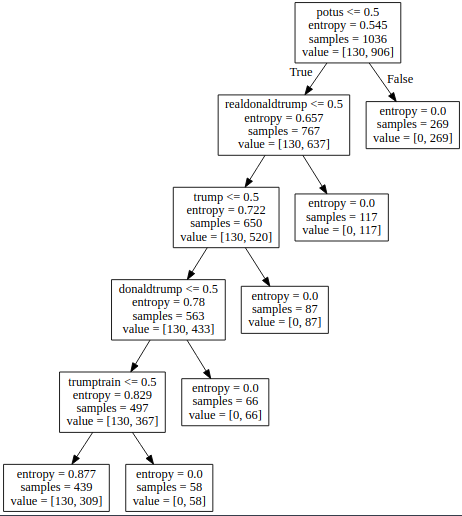
\includegraphics{tree_depth_5.png}
\caption{}
\end{figure}

    \subsubsection*{5) A description of a rule based on the
tree}\label{a-description-of-a-rule-based-on-the-tree}

    \begin{itemize}
\tightlist
\item
  If potus\textless{}=0.5:

  \begin{itemize}
  \tightlist
  \item
    If realdonaldtrump\textless{}=0.5:

    \begin{itemize}
    \tightlist
    \item
      If trump \textgreater{} 0.5:

      \begin{itemize}
      \tightlist
      \item
        then the tree reaches the leaf, value = \([0, 87]\), indicating
        that there are 87 tweets are categorized as \texttt{Relevant}
      \end{itemize}
    \end{itemize}
  \end{itemize}
\end{itemize}

    \subsubsection*{6) A short summary of your evaluation result using the
confusion
matrix}\label{a-short-summary-of-your-evaluation-result-using-the-confusion-matrix}

    \begin{Verbatim}[commandchars=\\\{\}]
{\color{incolor}In [{\color{incolor}58}]:} \PY{k}{def} \PY{n+nf}{plot\PYZus{}cm}\PY{p}{(}\PY{n}{cm}\PY{p}{,} \PY{n}{title}\PY{o}{=}\PY{l+s+s1}{\PYZsq{}}\PY{l+s+s1}{Confusion matrix}\PY{l+s+s1}{\PYZsq{}}\PY{p}{,} \PY{n}{cmap}\PY{o}{=}\PY{n}{plt}\PY{o}{.}\PY{n}{cm}\PY{o}{.}\PY{n}{Blues}\PY{p}{,} \PY{n}{classes}\PY{o}{=}\PY{p}{[}\PY{l+s+s1}{\PYZsq{}}\PY{l+s+s1}{Relevant}\PY{l+s+s1}{\PYZsq{}}\PY{p}{,} \PY{l+s+s1}{\PYZsq{}}\PY{l+s+s1}{Irrelevant}\PY{l+s+s1}{\PYZsq{}}\PY{p}{]}\PY{p}{)}\PY{p}{:}
             \PY{n+nb}{print}\PY{p}{(}\PY{n}{cm}\PY{p}{)}
             \PY{n}{plt}\PY{o}{.}\PY{n}{imshow}\PY{p}{(}\PY{n}{cm}\PY{p}{,} \PY{n}{interpolation}\PY{o}{=}\PY{l+s+s1}{\PYZsq{}}\PY{l+s+s1}{nearest}\PY{l+s+s1}{\PYZsq{}}\PY{p}{,} \PY{n}{cmap}\PY{o}{=}\PY{n}{cmap}\PY{p}{)}
             \PY{n}{plt}\PY{o}{.}\PY{n}{title}\PY{p}{(}\PY{n}{title}\PY{p}{)}
             \PY{n}{plt}\PY{o}{.}\PY{n}{colorbar}\PY{p}{(}\PY{p}{)}
             \PY{n}{tick\PYZus{}marks} \PY{o}{=} \PY{n}{np}\PY{o}{.}\PY{n}{arange}\PY{p}{(}\PY{n+nb}{len}\PY{p}{(}\PY{n}{classes}\PY{p}{)}\PY{p}{)}
             \PY{n}{target\PYZus{}names} \PY{o}{=} \PY{n}{classes}
             \PY{n}{plt}\PY{o}{.}\PY{n}{xticks}\PY{p}{(}\PY{n}{tick\PYZus{}marks}\PY{p}{,} \PY{n}{target\PYZus{}names}\PY{p}{,} \PY{n}{rotation}\PY{o}{=}\PY{l+m+mi}{45}\PY{p}{)}
             \PY{n}{plt}\PY{o}{.}\PY{n}{yticks}\PY{p}{(}\PY{n}{tick\PYZus{}marks}\PY{p}{,} \PY{n}{target\PYZus{}names}\PY{p}{)}
             \PY{n}{plt}\PY{o}{.}\PY{n}{tight\PYZus{}layout}\PY{p}{(}\PY{p}{)}
             \PY{n}{plt}\PY{o}{.}\PY{n}{ylabel}\PY{p}{(}\PY{l+s+s1}{\PYZsq{}}\PY{l+s+s1}{True label}\PY{l+s+s1}{\PYZsq{}}\PY{p}{)}
             \PY{n}{plt}\PY{o}{.}\PY{n}{xlabel}\PY{p}{(}\PY{l+s+s1}{\PYZsq{}}\PY{l+s+s1}{Predicted label}\PY{l+s+s1}{\PYZsq{}}\PY{p}{)}
         \PY{n}{plot\PYZus{}cm}\PY{p}{(}\PY{n}{confusion\PYZus{}matrix}\PY{p}{(}\PY{n}{y\PYZus{}test}\PY{p}{,} \PY{n}{y\PYZus{}pred}\PY{p}{)}\PY{p}{)}
\end{Verbatim}

    \begin{Verbatim}[commandchars=\\\{\}]
[[  0  33]
 [  0 227]]

    \end{Verbatim}

    \begin{center}
    \adjustimage{max size={0.5\linewidth}{0.5\paperheight}}{output_27_1.png}
    \end{center}
    { \hspace*{\fill} \\}
    
    \begin{Verbatim}[commandchars=\\\{\}]
{\color{incolor}In [{\color{incolor}56}]:} \PY{n+nb}{print}\PY{p}{(}\PY{l+s+s2}{\PYZdq{}}\PY{l+s+s2}{AUC(ROC): }\PY{l+s+s2}{\PYZdq{}} \PY{o}{+} \PY{n+nb}{str}\PY{p}{(}\PY{n}{metrics}\PY{o}{.}\PY{n}{roc\PYZus{}auc\PYZus{}score}\PY{p}{(}\PY{n}{y\PYZus{}test}\PY{p}{,} \PY{n}{y\PYZus{}pred}\PY{p}{)}\PY{p}{)}\PY{p}{)}
         \PY{n+nb}{print}\PY{p}{(}\PY{l+s+s2}{\PYZdq{}}\PY{l+s+s2}{Precision: }\PY{l+s+s2}{\PYZdq{}} \PY{o}{+} \PY{n+nb}{str}\PY{p}{(}\PY{n}{metrics}\PY{o}{.}\PY{n}{precision\PYZus{}score}\PY{p}{(}\PY{n}{y\PYZus{}test}\PY{p}{,} \PY{n}{y\PYZus{}pred}\PY{p}{)}\PY{p}{)}\PY{p}{)}
         \PY{n+nb}{print}\PY{p}{(}\PY{l+s+s2}{\PYZdq{}}\PY{l+s+s2}{Recall: }\PY{l+s+s2}{\PYZdq{}} \PY{o}{+} \PY{n+nb}{str}\PY{p}{(}\PY{n}{metrics}\PY{o}{.}\PY{n}{recall\PYZus{}score}\PY{p}{(}\PY{n}{y\PYZus{}test}\PY{p}{,} \PY{n}{y\PYZus{}pred}\PY{p}{)}\PY{p}{)}\PY{p}{)}
         \PY{n+nb}{print}\PY{p}{(}\PY{l+s+s2}{\PYZdq{}}\PY{l+s+s2}{F1 score: }\PY{l+s+s2}{\PYZdq{}} \PY{o}{+} \PY{n+nb}{str}\PY{p}{(}\PY{n}{metrics}\PY{o}{.}\PY{n}{f1\PYZus{}score}\PY{p}{(}\PY{n}{y\PYZus{}test}\PY{p}{,} \PY{n}{y\PYZus{}pred}\PY{p}{)}\PY{p}{)}\PY{p}{)}
\end{Verbatim}

    \begin{Verbatim}[commandchars=\\\{\}]
AUC(ROC): 0.5
Precision: 0.8730769230769231
Recall: 1.0
F1 score: 0.5322381930184805

    \end{Verbatim}

    Here we can see from the confusion matrix that the
\texttt{True\ Negative}=0, and \texttt{False\ Positive}=33, which means
all 33 \texttt{Irrelevant} tweets are categorized as \texttt{Relevant}.
Thus there appears to have a serious problem here: even with the
accuracy is decent, it is actually inflated. The reason for that is
because the proportion of \texttt{Relevant} tweets(\textbf{1133/1296})
is way larger than that of \texttt{Irrelevant}
tweets(\textbf{163/1296}), thus

\[accuracy = \frac{TP+TN}{TP+TN+FN+FP} = \frac{227}{260} = 87.3\%\]

In fact, with the task being to filter out the irrelevant tweets, this
classifier basically fails the task because of the unbalanced data.

    \subsubsection*{Possible fixes:}\label{possible-fixes}

\begin{itemize}
\tightlist
\item
  Resampling

  \begin{itemize}
  \tightlist
  \item
    Downsampling on the \texttt{Relevant} tweets
  \item
    Upsampling on the \texttt{Irrelevant} tweets
  \end{itemize}
\end{itemize}

    \begin{Verbatim}[commandchars=\\\{\}]
{\color{incolor}In [{\color{incolor}61}]:} \PY{k}{def} \PY{n+nf}{classify}\PY{p}{(}\PY{n}{X\PYZus{}train\PYZus{}vect}\PY{p}{,} \PY{n}{y\PYZus{}train}\PY{p}{,} \PY{n}{X\PYZus{}test\PYZus{}vect}\PY{p}{,} \PY{n}{y\PYZus{}test}\PY{p}{,} \PY{n}{model}\PY{p}{,} \PY{n}{vector}\PY{p}{)}\PY{p}{:}
             \PY{n}{clf}\PY{o}{.}\PY{n}{fit}\PY{p}{(}\PY{n}{X\PYZus{}train\PYZus{}vect}\PY{p}{,} \PY{n}{y\PYZus{}train}\PY{p}{)}
             \PY{n}{y\PYZus{}pred} \PY{o}{=} \PY{n}{clf}\PY{o}{.}\PY{n}{predict}\PY{p}{(}\PY{n}{X\PYZus{}test\PYZus{}vect}\PY{p}{)}
             \PY{n}{cross\PYZus{}val\PYZus{}s} \PY{o}{=} \PY{n}{np}\PY{o}{.}\PY{n}{mean}\PY{p}{(}\PY{p}{[}\PY{n}{cross\PYZus{}val\PYZus{}score}\PY{p}{(}\PY{n}{model}\PY{p}{,} \PY{n}{X\PYZus{}train\PYZus{}vect}\PY{p}{,} \PY{n}{y\PYZus{}train}\PY{p}{,} \PY{n}{cv}\PY{o}{=}\PY{l+m+mi}{8}\PY{p}{)}\PY{p}{]}\PY{p}{)}
             \PY{n+nb}{print}\PY{p}{(}\PY{l+s+s1}{\PYZsq{}}\PY{l+s+s1}{Cross\PYZus{}val\PYZus{}score: }\PY{l+s+si}{\PYZob{}\PYZcb{}}\PY{l+s+s1}{\PYZsq{}}\PY{o}{.}\PY{n}{format}\PY{p}{(}\PY{n}{cross\PYZus{}val\PYZus{}s}\PY{p}{)}\PY{p}{)}
             \PY{n+nb}{print}\PY{p}{(}\PY{l+s+s2}{\PYZdq{}}\PY{l+s+s2}{AUC(ROC): }\PY{l+s+s2}{\PYZdq{}} \PY{o}{+} \PY{n+nb}{str}\PY{p}{(}\PY{n}{metrics}\PY{o}{.}\PY{n}{roc\PYZus{}auc\PYZus{}score}\PY{p}{(}\PY{n}{y\PYZus{}test}\PY{p}{,} \PY{n}{y\PYZus{}pred}\PY{p}{)}\PY{p}{)}\PY{p}{)}
             \PY{n+nb}{print}\PY{p}{(}\PY{l+s+s2}{\PYZdq{}}\PY{l+s+s2}{Precision: }\PY{l+s+s2}{\PYZdq{}} \PY{o}{+} \PY{n+nb}{str}\PY{p}{(}\PY{n}{metrics}\PY{o}{.}\PY{n}{precision\PYZus{}score}\PY{p}{(}\PY{n}{y\PYZus{}test}\PY{p}{,} \PY{n}{y\PYZus{}pred}\PY{p}{)}\PY{p}{)}\PY{p}{)}
             \PY{n+nb}{print}\PY{p}{(}\PY{l+s+s2}{\PYZdq{}}\PY{l+s+s2}{Recall: }\PY{l+s+s2}{\PYZdq{}} \PY{o}{+} \PY{n+nb}{str}\PY{p}{(}\PY{n}{metrics}\PY{o}{.}\PY{n}{recall\PYZus{}score}\PY{p}{(}\PY{n}{y\PYZus{}test}\PY{p}{,} \PY{n}{y\PYZus{}pred}\PY{p}{)}\PY{p}{)}\PY{p}{)}
             \PY{n+nb}{print}\PY{p}{(}\PY{l+s+s2}{\PYZdq{}}\PY{l+s+s2}{F1 score: }\PY{l+s+s2}{\PYZdq{}} \PY{o}{+} \PY{n+nb}{str}\PY{p}{(}\PY{n}{metrics}\PY{o}{.}\PY{n}{f1\PYZus{}score}\PY{p}{(}\PY{n}{y\PYZus{}test}\PY{p}{,} \PY{n}{y\PYZus{}pred}\PY{p}{)}\PY{p}{)}\PY{p}{)}
             \PY{n+nb}{print}\PY{p}{(}\PY{n}{metrics}\PY{o}{.}\PY{n}{confusion\PYZus{}matrix}\PY{p}{(}\PY{n}{y\PYZus{}test}\PY{p}{,} \PY{n}{y\PYZus{}pred}\PY{p}{)}\PY{p}{)}
             \PY{n}{plt}\PY{o}{.}\PY{n}{figure}\PY{p}{(}\PY{n}{figsize}\PY{o}{=}\PY{p}{(}\PY{l+m+mi}{5}\PY{p}{,}\PY{l+m+mi}{5}\PY{p}{)}\PY{p}{)}
             \PY{n}{plot\PYZus{}cm}\PY{p}{(}\PY{n}{metrics}\PY{o}{.}\PY{n}{confusion\PYZus{}matrix}\PY{p}{(}\PY{n}{y\PYZus{}test}\PY{p}{,} \PY{n}{y\PYZus{}pred}\PY{p}{)}\PY{p}{)}
             \PY{n}{plt}\PY{o}{.}\PY{n}{show}\PY{p}{(}\PY{p}{)}
             \PY{k}{return} \PY{n}{cross\PYZus{}val\PYZus{}s}
\end{Verbatim}

    \subsubsection*{\texorpdfstring{Experiment 1: Downsample the
\texttt{Relevant}
data}{Experiment 1: Downsample the Relevant data}}\label{experiment-1-downsample-the-relevant-data}

    \begin{Verbatim}[commandchars=\\\{\}]
{\color{incolor}In [{\color{incolor}62}]:} \PY{k}{def} \PY{n+nf}{undersample}\PY{p}{(}\PY{n}{data}\PY{p}{,} \PY{n}{percentage}\PY{p}{,} \PY{n}{vector}\PY{p}{)}\PY{p}{:}
             \PY{n}{relevant\PYZus{}idx} \PY{o}{=} \PY{n}{tagged}\PY{p}{[}\PY{n}{tagged}\PY{o}{.}\PY{n}{Relevant}\PY{o}{==}\PY{l+m+mi}{1}\PY{p}{]}\PY{o}{.}\PY{n}{index}
             \PY{n}{irrelevant\PYZus{}idx} \PY{o}{=} \PY{n}{tagged}\PY{p}{[}\PY{n}{tagged}\PY{o}{.}\PY{n}{Relevant}\PY{o}{==}\PY{l+m+mi}{0}\PY{p}{]}\PY{o}{.}\PY{n}{index}
             \PY{n}{undersample\PYZus{}relevant\PYZus{}idx} \PY{o}{=} \PY{n}{np}\PY{o}{.}\PY{n}{array}\PY{p}{(}\PY{n}{np}\PY{o}{.}\PY{n}{random}\PY{o}{.}\PY{n}{choice}\PY{p}{(}\PY{n}{relevant\PYZus{}idx}\PY{p}{,}\PY{p}{(}\PY{n+nb}{int}\PY{p}{(}\PY{n}{percentage}\PY{o}{*}\PY{n+nb}{len}\PY{p}{(}\PY{n}{irrelevant\PYZus{}idx}\PY{p}{)}\PY{p}{)}\PY{p}{)}\PY{p}{,}\PY{n}{replace}\PY{o}{=}\PY{k+kc}{False}\PY{p}{)}\PY{p}{)}
             \PY{n}{undersample\PYZus{}idx}\PY{o}{=} \PY{n}{np}\PY{o}{.}\PY{n}{concatenate}\PY{p}{(}\PY{p}{[}\PY{n}{irrelevant\PYZus{}idx}\PY{p}{,} \PY{n}{undersample\PYZus{}relevant\PYZus{}idx}\PY{p}{]}\PY{p}{)}
             \PY{n}{undersample\PYZus{}data} \PY{o}{=} \PY{n}{tagged}\PY{o}{.}\PY{n}{iloc}\PY{p}{[}\PY{n}{undersample\PYZus{}idx}\PY{p}{,}\PY{p}{:}\PY{p}{]}
             \PY{n+nb}{print}\PY{p}{(}\PY{l+s+s1}{\PYZsq{}}\PY{l+s+s1}{There are }\PY{l+s+si}{\PYZob{}\PYZcb{}}\PY{l+s+s1}{ relevant tweets.}\PY{l+s+se}{\PYZbs{}n}\PY{l+s+s1}{ There are }\PY{l+s+si}{\PYZob{}\PYZcb{}}\PY{l+s+s1}{ irrelevant tweets.}\PY{l+s+s1}{\PYZsq{}}\PY{o}{.}\PY{n}{format}\PY{p}{(}\PY{n+nb}{len}\PY{p}{(}\PY{n}{undersample\PYZus{}data}\PY{p}{[}\PY{n}{undersample\PYZus{}data}\PY{o}{.}\PY{n}{Relevant}\PY{o}{==}\PY{l+m+mi}{1}\PY{p}{]}\PY{p}{)}\PY{p}{,} 
                                                                                            \PY{n+nb}{len}\PY{p}{(}\PY{n}{undersample\PYZus{}data}\PY{p}{[}\PY{n}{undersample\PYZus{}data}\PY{o}{.}\PY{n}{Relevant}\PY{o}{==}\PY{l+m+mi}{0}\PY{p}{]}\PY{p}{)}\PY{p}{)}\PY{p}{)}
             \PY{n}{X\PYZus{}train}\PY{p}{,} \PY{n}{X\PYZus{}test}\PY{p}{,} \PY{n}{y\PYZus{}train}\PY{p}{,} \PY{n}{y\PYZus{}test} \PY{o}{=} \PY{n}{train\PYZus{}test\PYZus{}split}\PY{p}{(}\PY{n}{undersample\PYZus{}data}\PY{o}{.}\PY{n}{text}\PY{p}{,} \PY{n}{undersample\PYZus{}data}\PY{o}{.}\PY{n}{Relevant}\PY{p}{,} \PY{n}{test\PYZus{}size}\PY{o}{=}\PY{l+m+mf}{0.2}\PY{p}{,} \PY{n}{random\PYZus{}state}\PY{o}{=}\PY{l+m+mi}{100}\PY{p}{)}
             \PY{n}{X\PYZus{}train\PYZus{}vect} \PY{o}{=} \PY{n}{vector}\PY{o}{.}\PY{n}{fit\PYZus{}transform}\PY{p}{(}\PY{n}{X\PYZus{}train}\PY{p}{)}\PY{o}{.}\PY{n}{todense}\PY{p}{(}\PY{p}{)}
             \PY{n}{X\PYZus{}test\PYZus{}vect} \PY{o}{=} \PY{n}{vector}\PY{o}{.}\PY{n}{transform}\PY{p}{(}\PY{n}{X\PYZus{}test}\PY{p}{)}
             \PY{n}{plt}\PY{o}{.}\PY{n}{figure}\PY{p}{(}\PY{n}{figsize}\PY{o}{=}\PY{p}{(}\PY{l+m+mi}{5}\PY{p}{,}\PY{l+m+mi}{5}\PY{p}{)}\PY{p}{)}
             \PY{n}{sns}\PY{o}{.}\PY{n}{countplot}\PY{p}{(}\PY{l+s+s2}{\PYZdq{}}\PY{l+s+s2}{Relevant}\PY{l+s+s2}{\PYZdq{}}\PY{p}{,}\PY{n}{data}\PY{o}{=}\PY{n}{undersample\PYZus{}data}\PY{p}{)}
             \PY{n}{plt}\PY{o}{.}\PY{n}{show}\PY{p}{(}\PY{p}{)}
             \PY{k}{return} \PY{n}{X\PYZus{}train\PYZus{}vect}\PY{p}{,} \PY{n}{X\PYZus{}test\PYZus{}vect}\PY{p}{,} \PY{n}{y\PYZus{}train}\PY{p}{,} \PY{n}{y\PYZus{}test}
\end{Verbatim}

    \begin{Verbatim}[commandchars=\\\{\}]
{\color{incolor}In [{\color{incolor}66}]:} \PY{n}{cross\PYZus{}val\PYZus{}scores}\PY{o}{=}\PY{p}{[}\PY{p}{]}
         \PY{k}{for} \PY{n}{percentage} \PY{o+ow}{in} \PY{n}{np}\PY{o}{.}\PY{n}{arange}\PY{p}{(}\PY{l+m+mi}{1}\PY{p}{,} \PY{l+m+mi}{4}\PY{p}{,} \PY{l+m+mf}{0.5}\PY{p}{)}\PY{p}{:}
             \PY{n}{X\PYZus{}train\PYZus{}vect}\PY{p}{,} \PY{n}{X\PYZus{}test\PYZus{}vect}\PY{p}{,} \PY{n}{y\PYZus{}train}\PY{p}{,} \PY{n}{y\PYZus{}test} \PY{o}{=} \PY{n}{undersample}\PY{p}{(}\PY{n}{tagged}\PY{p}{,} \PY{n}{percentage}\PY{p}{,} \PY{n}{vect}\PY{p}{)}
             \PY{n}{cross\PYZus{}val\PYZus{}s} \PY{o}{=} \PY{n}{classify}\PY{p}{(}\PY{n}{X\PYZus{}train\PYZus{}vect}\PY{o}{=}\PY{n}{X\PYZus{}train\PYZus{}vect}\PY{p}{,}
                 \PY{n}{X\PYZus{}test\PYZus{}vect}\PY{o}{=}\PY{n}{X\PYZus{}test\PYZus{}vect}\PY{p}{,}
                 \PY{n}{y\PYZus{}train} \PY{o}{=}\PY{n}{y\PYZus{}train}\PY{p}{,}
                 \PY{n}{y\PYZus{}test}\PY{o}{=}\PY{n}{y\PYZus{}test}\PY{p}{,}
                 \PY{n}{model}\PY{o}{=}\PY{n}{clf}\PY{p}{,}
                 \PY{n}{vector}\PY{o}{=}\PY{n}{vect}\PY{p}{)}
             \PY{n}{cross\PYZus{}val\PYZus{}scores}\PY{o}{.}\PY{n}{append}\PY{p}{(}\PY{n}{cross\PYZus{}val\PYZus{}s}\PY{p}{)}
         \PY{n}{plt}\PY{o}{.}\PY{n}{figure}\PY{p}{(}\PY{n}{figsize}\PY{o}{=}\PY{p}{(}\PY{l+m+mi}{5}\PY{p}{,}\PY{l+m+mi}{5}\PY{p}{)}\PY{p}{)}
         \PY{n}{plt}\PY{o}{.}\PY{n}{plot}\PY{p}{(}\PY{n}{np}\PY{o}{.}\PY{n}{arange}\PY{p}{(}\PY{l+m+mi}{1}\PY{p}{,}\PY{l+m+mi}{4}\PY{p}{,}\PY{l+m+mf}{0.5}\PY{p}{)}\PY{p}{,} \PY{n}{cross\PYZus{}val\PYZus{}scores}\PY{p}{)}
         \PY{n}{plt}\PY{o}{.}\PY{n}{scatter}\PY{p}{(}\PY{n}{np}\PY{o}{.}\PY{n}{arange}\PY{p}{(}\PY{l+m+mi}{1}\PY{p}{,}\PY{l+m+mi}{4}\PY{p}{,}\PY{l+m+mf}{0.5}\PY{p}{)}\PY{p}{,} \PY{n}{cross\PYZus{}val\PYZus{}scores}\PY{p}{,} \PY{n}{c}\PY{o}{=}\PY{l+s+s1}{\PYZsq{}}\PY{l+s+s1}{r}\PY{l+s+s1}{\PYZsq{}}\PY{p}{)}
         \PY{n}{plt}\PY{o}{.}\PY{n}{show}\PY{p}{(}\PY{p}{)}
\end{Verbatim}

    \begin{Verbatim}[commandchars=\\\{\}]
There are 163 relevant tweets.
 There are 163 irrelevant tweets.

    \end{Verbatim}

    \begin{center}
    \adjustimage{max size={0.5\linewidth}{0.5\paperheight}}{output_34_1.png}
    \end{center}
    { \hspace*{\fill} \\}
    
    \begin{Verbatim}[commandchars=\\\{\}]
Cross\_val\_score: 0.8041758308895406
AUC(ROC): 0.8157894736842105
Precision: 1.0
Recall: 0.631578947368421
F1 score: 0.7741935483870968
[[28  0]
 [14 24]]
[[28  0]
 [14 24]]

    \end{Verbatim}

    \begin{center}
    \adjustimage{max size={0.5\linewidth}{0.5\paperheight}}{output_34_3.png}
    \end{center}
    { \hspace*{\fill} \\}
    
    \begin{Verbatim}[commandchars=\\\{\}]
There are 244 relevant tweets.
 There are 163 irrelevant tweets.

    \end{Verbatim}

    \begin{center}
    \adjustimage{max size={0.5\linewidth}{0.5\paperheight}}{output_34_5.png}
    \end{center}
    { \hspace*{\fill} \\}
    
    \begin{Verbatim}[commandchars=\\\{\}]
Cross\_val\_score: 0.824130315822389
AUC(ROC): 0.8773584905660378
Precision: 1.0
Recall: 0.7547169811320755
F1 score: 0.8602150537634409
[[29  0]
 [13 40]]
[[29  0]
 [13 40]]

    \end{Verbatim}

    \begin{center}
    \adjustimage{max size={0.5\linewidth}{0.5\paperheight}}{output_34_7.png}
    \end{center}
    { \hspace*{\fill} \\}
    
    \begin{Verbatim}[commandchars=\\\{\}]
There are 326 relevant tweets.
 There are 163 irrelevant tweets.

    \end{Verbatim}

    \begin{center}
    \adjustimage{max size={0.5\linewidth}{0.5\paperheight}}{output_34_9.png}
    \end{center}
    { \hspace*{\fill} \\}
    
    \begin{Verbatim}[commandchars=\\\{\}]
Cross\_val\_score: 0.7495153061224489
AUC(ROC): 0.875
Precision: 1.0
Recall: 0.75
F1 score: 0.8571428571428571
[[30  0]
 [17 51]]
[[30  0]
 [17 51]]

    \end{Verbatim}

    \begin{center}
    \adjustimage{max size={0.5\linewidth}{0.5\paperheight}}{output_34_11.png}
    \end{center}
    { \hspace*{\fill} \\}
    
    \begin{Verbatim}[commandchars=\\\{\}]
There are 407 relevant tweets.
 There are 163 irrelevant tweets.

    \end{Verbatim}

    \begin{center}
    \adjustimage{max size={0.5\linewidth}{0.5\paperheight}}{output_34_13.png}
    \end{center}
    { \hspace*{\fill} \\}
    
    \begin{Verbatim}[commandchars=\\\{\}]
Cross\_val\_score: 0.7327586206896551
AUC(ROC): 0.8192771084337349
Precision: 1.0
Recall: 0.6385542168674698
F1 score: 0.7794117647058824
[[31  0]
 [30 53]]
[[31  0]
 [30 53]]

    \end{Verbatim}

    \begin{center}
    \adjustimage{max size={0.5\linewidth}{0.5\paperheight}}{output_34_15.png}
    \end{center}
    { \hspace*{\fill} \\}
    
    \begin{Verbatim}[commandchars=\\\{\}]
There are 489 relevant tweets.
 There are 163 irrelevant tweets.

    \end{Verbatim}

    \begin{center}
    \adjustimage{max size={0.5\linewidth}{0.5\paperheight}}{output_34_17.png}
    \end{center}
    { \hspace*{\fill} \\}
    
    \begin{Verbatim}[commandchars=\\\{\}]
Cross\_val\_score: 0.7214352054195804
AUC(ROC): 0.5
Precision: 0.7557251908396947
Recall: 1.0
F1 score: 0.8608695652173913
[[ 0 32]
 [ 0 99]]
[[ 0 32]
 [ 0 99]]

    \end{Verbatim}

    \begin{center}
    \adjustimage{max size={0.5\linewidth}{0.5\paperheight}}{output_34_19.png}
    \end{center}
    { \hspace*{\fill} \\}
    
    \begin{Verbatim}[commandchars=\\\{\}]
There are 570 relevant tweets.
 There are 163 irrelevant tweets.

    \end{Verbatim}

    \begin{center}
    \adjustimage{max size={0.5\linewidth}{0.5\paperheight}}{output_34_21.png}
    \end{center}
    { \hspace*{\fill} \\}
    
    \begin{Verbatim}[commandchars=\\\{\}]
Cross\_val\_score: 0.7850140380106133
AUC(ROC): 0.5
Precision: 0.7482993197278912
Recall: 1.0
F1 score: 0.8560311284046693
[[  0  37]
 [  0 110]]
[[  0  37]
 [  0 110]]

    \end{Verbatim}

    \begin{center}
    \adjustimage{max size={0.5\linewidth}{0.5\paperheight}}{output_34_23.png}
    \end{center}
    { \hspace*{\fill} \\}
    
    \begin{center}
    \adjustimage{max size={0.5\linewidth}{0.5\paperheight}}{output_34_24.png}
    \end{center}
    { \hspace*{\fill} \\}
    
    \subsubsection*{\texorpdfstring{Experiment 2: Upsample the
\texttt{Irrelevant}
data}{Experiment 2: Upsample the Irrelevant data}}\label{experiment-2-upsample-the-irrelevant-data}

    \begin{Verbatim}[commandchars=\\\{\}]
{\color{incolor}In [{\color{incolor}64}]:} \PY{k}{def} \PY{n+nf}{oversample}\PY{p}{(}\PY{n}{data}\PY{p}{,} \PY{n}{vector}\PY{p}{)}\PY{p}{:}
             \PY{n}{os} \PY{o}{=} \PY{n}{SMOTE}\PY{p}{(}\PY{n}{random\PYZus{}state}\PY{o}{=}\PY{l+m+mi}{0}\PY{p}{)}
             \PY{n}{X\PYZus{}train}\PY{p}{,} \PY{n}{X\PYZus{}test}\PY{p}{,} \PY{n}{y\PYZus{}train}\PY{p}{,} \PY{n}{y\PYZus{}test} \PY{o}{=} \PY{n}{train\PYZus{}test\PYZus{}split}\PY{p}{(}\PY{n}{data}\PY{o}{.}\PY{n}{text}\PY{p}{,} \PY{n}{data}\PY{o}{.}\PY{n}{Relevant}\PY{p}{,} \PY{n}{test\PYZus{}size}\PY{o}{=}\PY{l+m+mf}{0.2}\PY{p}{,} \PY{n}{random\PYZus{}state}\PY{o}{=}\PY{l+m+mi}{100}\PY{p}{)}
             \PY{n}{X\PYZus{}train\PYZus{}vect} \PY{o}{=} \PY{n}{vector}\PY{o}{.}\PY{n}{fit\PYZus{}transform}\PY{p}{(}\PY{n}{X\PYZus{}train}\PY{p}{)}\PY{o}{.}\PY{n}{todense}\PY{p}{(}\PY{p}{)}
             \PY{n}{X\PYZus{}test\PYZus{}vect} \PY{o}{=} \PY{n}{vector}\PY{o}{.}\PY{n}{transform}\PY{p}{(}\PY{n}{X\PYZus{}test}\PY{p}{)}
             \PY{n}{os\PYZus{}X\PYZus{}train}\PY{p}{,} \PY{n}{os\PYZus{}y\PYZus{}train} \PY{o}{=} \PY{n}{os}\PY{o}{.}\PY{n}{fit\PYZus{}sample}\PY{p}{(}\PY{n}{X\PYZus{}train\PYZus{}vect}\PY{p}{,} \PY{n}{y\PYZus{}train}\PY{p}{)}
             \PY{k}{return} \PY{n}{os\PYZus{}X\PYZus{}train}\PY{p}{,} \PY{n}{X\PYZus{}test\PYZus{}vect}\PY{p}{,} \PY{n}{os\PYZus{}y\PYZus{}train}\PY{p}{,} \PY{n}{y\PYZus{}test}
\end{Verbatim}

    \begin{Verbatim}[commandchars=\\\{\}]
{\color{incolor}In [{\color{incolor}65}]:} \PY{n}{X\PYZus{}train\PYZus{}vect}\PY{p}{,} \PY{n}{X\PYZus{}test\PYZus{}vect}\PY{p}{,} \PY{n}{y\PYZus{}train}\PY{p}{,} \PY{n}{y\PYZus{}test} \PY{o}{=} \PY{n}{oversample}\PY{p}{(}\PY{n}{tagged}\PY{p}{,} \PY{n}{vect}\PY{p}{)}
         \PY{n}{classify}\PY{p}{(}\PY{n}{X\PYZus{}train\PYZus{}vect}\PY{o}{=}\PY{n}{X\PYZus{}train\PYZus{}vect}\PY{p}{,}
                 \PY{n}{X\PYZus{}test\PYZus{}vect}\PY{o}{=}\PY{n}{X\PYZus{}test\PYZus{}vect}\PY{p}{,}
                 \PY{n}{y\PYZus{}train} \PY{o}{=}\PY{n}{y\PYZus{}train}\PY{p}{,}
                 \PY{n}{y\PYZus{}test}\PY{o}{=}\PY{n}{y\PYZus{}test}\PY{p}{,}
                 \PY{n}{model}\PY{o}{=}\PY{n}{clf}\PY{p}{,}
                 \PY{n}{vector}\PY{o}{=}\PY{n}{vect}\PY{p}{)}
\end{Verbatim}

    \begin{Verbatim}[commandchars=\\\{\}]
Cross\_val\_score: 0.8281613879832324
AUC(ROC): 0.8223684210526316
Precision: 1.0
Recall: 0.6447368421052632
F1 score: 0.7839999999999999
[[ 32   0]
 [ 81 147]]
[[ 32   0]
 [ 81 147]]

    \end{Verbatim}

    \begin{center}
    \adjustimage{max size={0.5\linewidth}{0.5\paperheight}}{output_37_1.png}
    \end{center}
    { \hspace*{\fill} \\}
    
\begin{Verbatim}[commandchars=\\\{\}]
{\color{outcolor}Out[{\color{outcolor}65}]:} 0.8281613879832324
\end{Verbatim}
            

    % Add a bibliography block to the postdoc
    
    
    
    \end{document}
